\chapter{O ar ao nosso redor}\label{ch:g2:air-around-us}

Balance a mão depressa na frente do rosto: alguma coisa macia roça a
sua bochecha. Você não consegue vê-la, agarrá-la nem guardá-la numa
gaveta --- e mesmo assim ela enche todos os cômodos, todas as
garrafas, todos os pátios da Terra. Este capítulo é sobre o \omterm{def:g2:air-around-us:air}{ar}: o
material invisível no fundo do qual vivemos.

\section{O ar é mesmo alguma coisa?}

\begin{definition}[Ar]\label{def:g2:air-around-us:air}
O \emph{ar}\index{ar} é o material invisível que está em toda parte
ao nosso redor. Ele não tem cor, não tem cheiro próprio e a \omterm{def:g1:light-and-shadows:source}{luz} o
atravessa direto --- e é por isso que esquecemos que ele está ali.
Mas ele é material de verdade, como as experiências deste capítulo
vão provar, e é precioso: cada respiração sua é um gole dele.
\end{definition}

\begin{example}[Experimente: pegue um pouco de ar]\label{ex:g2:air-around-us:catch}
Abra bem um saco plástico, passe-o pelo cômodo e feche-o torcendo a
boca. O saco fica inchado como uma almofada --- aperte: ele empurra
de volta! Está claro que há alguma coisa presa lá dentro. Abra uma
pontinha e aperte de novo: você sente o prisioneiro invisível
escorrendo por cima dos seus dedos. Um saco ``vazio'', cheio de nada,
não conseguiria empurrar de volta.
\end{example}

\begin{example}[Onde o ar se mostra]\label{ex:g2:air-around-us:shows}
O \omterm{def:g2:air-around-us:air}{ar} é invisível, mas os truques dele não são: ele tremeluz acima de
uma estrada quente, levanta pipas, faz as folhas farfalharem e produz
bolhas em todo lugar por onde escapa debaixo d'água. Assopre por um
canudinho dentro do seu copo: cada bolha prateada é um pacotinho de
\omterm{def:g2:air-around-us:air}{ar} a caminho da superfície.
\end{example}

\section{O ar ocupa lugar}

\begin{method}[O mergulho do papel seco]\label{met:g2:air-around-us:drytowel}
Um truque de mágica que é pura física --- faça sobre uma bacia.
\begin{enumerate}
  \item Enfie uma folha de papel-toalha seca bem apertada no fundo de
        um copo, de modo que ela não caia;
  \item vire o copo exatamente de cabeça para baixo;
  \item empurre-o direto para dentro de uma bacia de água, mais fundo
        que o copo inteiro, sem inclinar;
  \item puxe-o direto para fora e toque no papel.
\end{enumerate}
O papel está perfeitamente seco! O copo nunca esteve vazio: ele
estava cheio de \omterm{def:g2:air-around-us:air}{ar}, e o \omterm{def:g2:air-around-us:air}{ar} preso guardou o lugar dele, então a água
não conseguiu entrar.
\end{method}

\begin{omfigure}
\begin{tikzpicture}[scale=0.85]
  % basin of water
  \draw[thick] (0,3.2) -- (0,0) -- (9.0,0) -- (9.0,3.2);
  \fill[omDef, opacity=0.15] (0,0) rectangle (9.0,2.7);
  \draw[omDef, thick] (0,2.7) -- (9.0,2.7);
  % the upside-down glass, pushed fully under
  \fill[white] (2.75,0.42) rectangle (4.45,2.28);
  \fill[omDef, opacity=0.15] (2.75,0.42) rectangle (4.45,0.85);
  \draw[line width=2.4pt, omExo!75]
    (2.7,0.4) -- (2.7,2.3) -- (4.5,2.3) -- (4.5,0.4);
  \draw[omDef, thick] (2.75,0.85) -- (4.45,0.85);
  \draw[thick, fill=omMeth, fill opacity=0.5]
    (2.95,1.75) rectangle (4.25,2.15);
  \node[font=\footnotesize, align=center] at (3.6,1.4)
    {ar\\preso};
  % leaders to labels in the open
  \draw[omExo!80, thin] (4.28,1.98) -- (5.4,3.62);
  \node[right, font=\small] at (5.45,3.62) {o papel, perfeitamente seco};
  \draw[omExo!80, thin] (4.45,0.85) -- (5.8,-0.42);
  \node[right, font=\small] at (5.85,-0.42)
    {a água para aqui: o ar guarda o lugar dele};
\end{tikzpicture}

{\small O mergulho do papel seco: o copo de cabeça para baixo está
cheio de \omterm{def:g2:air-around-us:air}{ar}, e duas coisas não podem estar no mesmo lugar ao mesmo
tempo.}
\end{omfigure}

\begin{example}[A garrafa que faz glub]\label{ex:g2:air-around-us:glug}
Empurre uma garrafa ``vazia'' de boca para baixo dentro da bacia e
incline um pouquinho: glub, glub, glub --- bolhas prateadas grandes
disparam para a superfície, e a água toma o lugar delas lá dentro. A
garrafa estava cheia de \omterm{def:g2:air-around-us:air}{ar}; a água só consegue entrar na mesma
velocidade com que o \omterm{def:g2:air-around-us:air}{ar} sai. Aquele glub na pia da cozinha é o som do
\omterm{def:g2:air-around-us:air}{ar} e da água trocando de lugar.
\end{example}

\begin{omfigure}
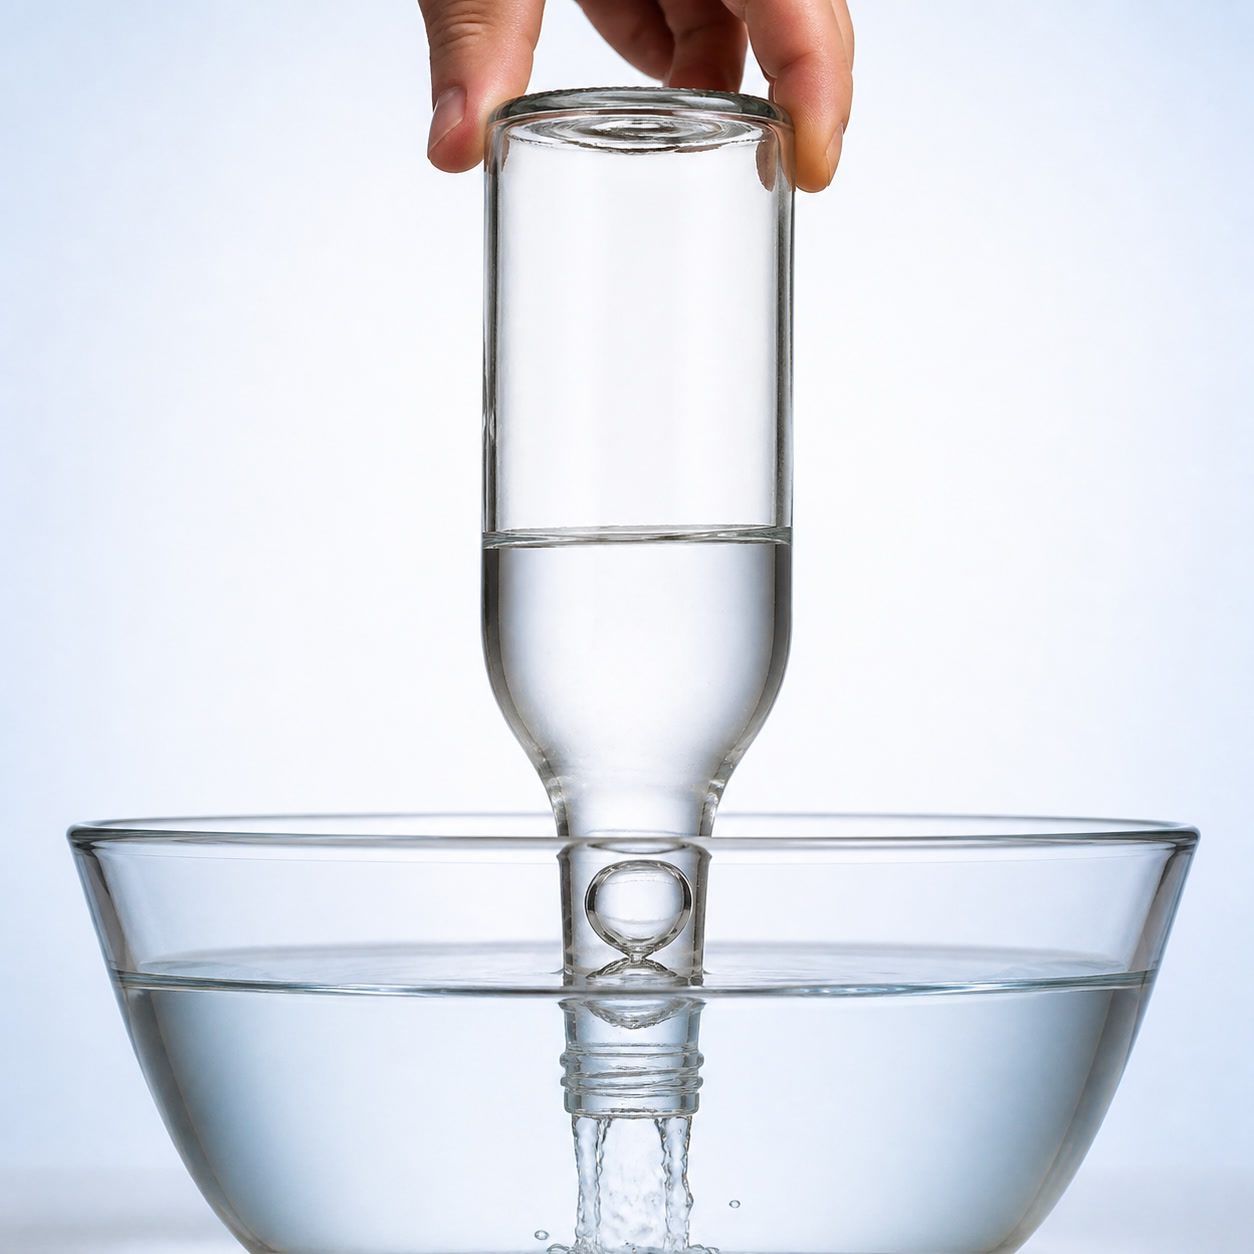
\includegraphics[width=0.42\linewidth]{images/book1/ai/g2-air-glugging-bottle.jpg}

{\small A garrafa que faz glub: enquanto a água sai, bolhas grandes de \omterm{def:g2:air-around-us:air}{ar} abrem caminho para dentro --- o espaço ``vazio'' precisa ser preenchido.}
\end{omfigure}

\begin{remark}[Não existe garrafa vazia]\label{rem:g2:air-around-us:noempty}
De agora em diante, desconfie da palavra ``vazio''. A garrafa vazia,
o copo vazio, a caixa vazia: todos cheios de \omterm{def:g2:air-around-us:air}{ar}, até a boca.
Realmente vazio --- sem absolutamente nada dentro, nem mesmo \omterm{def:g2:air-around-us:air}{ar} ---
é muito difícil de conseguir, e um dia você vai conhecer o nome
estranho que os cientistas dão a isso.
\end{remark}

\section{O ar empurra}

\begin{definition}[Vento]\label{def:g2:air-around-us:wind}
\emph{Vento}\index{vento} é \omterm{def:g2:air-around-us:air}{ar} em movimento. O \omterm{def:g2:air-around-us:air}{ar} parado não roça
ninguém; o \omterm{def:g2:air-around-us:air}{ar} em movimento empurra tudo o que estiver no caminho dele
--- de leve num dia de brisa, com força suficiente numa tempestade
para entortar árvores.
\end{definition}

\begin{example}[O ar trabalhando]\label{ex:g2:air-around-us:work}
O \omterm{def:g2:air-around-us:air}{ar} em movimento faz serviços de verdade: ele enche as velas dos
barcos, gira cataventos, seca a roupa e sustenta as pipas. Você mesmo
fabrica \omterm{def:g2:air-around-us:wind}{vento} toda vez que assopra uma vela de aniversário --- o seu
sopro é uma rajada particular e pequena, forte o bastante para
empurrar a chama para fora do pavio.
\end{example}

\begin{example}[Experimente: o balão a jato]\label{ex:g2:air-around-us:balloon}
Encha um balão de \omterm{def:g2:air-around-us:air}{ar} e segure o bico fechado. Lá dentro, \omterm{def:g2:air-around-us:air}{ar}
espremido está esperando. Solte: o \omterm{def:g2:air-around-us:air}{ar} sai correndo para trás, e o
balão dispara para a frente pelo cômodo, sacudindo doido. O \omterm{def:g2:air-around-us:air}{ar} que
escapa empurra o balão --- um priminho pequeno do jeito como o gás
espremido para fora empurra os foguetes de verdade.
\end{example}

\begin{omfigure}
\begin{tikzpicture}[scale=0.85]
  % balloon body and its open neck
  \draw[thick, fill=omThm, fill opacity=0.3]
    (4.75,1.3) ellipse (1.4 and 0.95);
  \draw[thick, fill=omThm, fill opacity=0.3]
    (3.44,1.55) .. controls (3.2,1.48) .. (3.02,1.52)
    -- (3.02,1.08) .. controls (3.2,1.12) .. (3.44,1.05) -- cycle;
  % escaping air, fanning backward
  \draw[-Stealth, omDef, thick] (2.85,1.48) -- (1.65,1.66);
  \draw[-Stealth, omDef, thick] (2.85,1.3) -- (1.55,1.3);
  \draw[-Stealth, omDef, thick] (2.85,1.12) -- (1.65,0.94);
  \node[below, font=\small, omDef] at (1.85,0.66) {o ar sai correndo};
  % the flight
  \draw[-Stealth, very thick, omThm] (6.4,1.3) -- (8.1,1.3);
  \node[below right, font=\small, omThm] at (6.3,1.05)
    {o balão dispara para a frente};
\end{tikzpicture}

{\small O balão a jato: o \omterm{def:g2:air-around-us:air}{ar} escapando para um lado empurra o balão
para o outro lado.}
\end{omfigure}

\begin{remark}[O ar é precioso]\label{rem:g2:air-around-us:breathe}
O empurrão mais importante de todos acontece caladinho no seu peito:
a cada respiração, o \omterm{def:g2:air-around-us:air}{ar} entra, o seu corpo guarda um pouquinho do que
precisa e o resto sai. Pessoas, gatos, pássaros e até os peixes (que
sorvem o \omterm{def:g2:air-around-us:air}{ar} escondido na água) precisam da sua parte. Invisível não
quer dizer sem importância --- com o \omterm{def:g2:air-around-us:air}{ar}, quer dizer justamente o
contrário.
\end{remark}

\section{Exercícios}

\begin{exercise}[$\star$]\label{exo:g2:air-around-us:1}
Diga três pistas, vistas nesta semana, de que o \omterm{def:g2:air-around-us:air}{ar} é real --- sem
usar nenhuma experiência de livro.
\end{exercise}

\begin{exercise}[$\star$]\label{exo:g2:air-around-us:2}
Por que o saco fechado do \cref{ex:g2:air-around-us:catch} empurra de
volta quando você aperta? O que tem lá dentro?
\end{exercise}

\begin{exercise}[$\star$]\label{exo:g2:air-around-us:3}
No mergulho do papel seco, por que a água não chega até o papel? Diga
com as palavras do capítulo: quem guarda o lugar?
\end{exercise}

\begin{exercise}[$\star$]\label{exo:g2:air-around-us:4}
O que você \emph{não} pode fazer com o copo durante o mergulho do
papel seco, e o que aconteceria com o papel se fizesse?
\end{exercise}

\begin{exercise}[$\star$]\label{exo:g2:air-around-us:5}
O que é o glub-glub de uma garrafa enchendo debaixo d'água? O que sai,
o que entra e por que os dois precisam se revezar?
\end{exercise}

\begin{exercise}[$\star$]\label{exo:g2:air-around-us:6}
``Me passe a garrafa vazia.'' O que há de verdade dentro de uma
garrafa vazia? (Veja a \cref{rem:g2:air-around-us:noempty}.)
\end{exercise}

\begin{exercise}[$\star$]\label{exo:g2:air-around-us:7}
O que é o \omterm{def:g2:air-around-us:wind}{vento}, nas palavras da \cref{def:g2:air-around-us:wind}? Dê
dois serviços que o \omterm{def:g2:air-around-us:air}{ar} em movimento faz.
\end{exercise}

\begin{exercise}[$\star$]\label{exo:g2:air-around-us:8}
Quando o balão a jato voa, para que lado o \omterm{def:g2:air-around-us:air}{ar} sai correndo e para que
lado vai o balão?
\end{exercise}

\begin{exercise}[$\star\star$]\label{exo:g2:air-around-us:9}
Um funil está encaixado justinho no gargalo de uma garrafa, vedado em
toda a volta com massinha adesiva. Ana despeja água no funil --- e,
depois de um golinho, a água simplesmente fica parada no funil,
recusando-se a descer para a garrafa. Explique o que a bloqueia e
proponha a solução de um segundo.
\end{exercise}

\begin{exercise}[$\star\star$]\label{exo:g2:air-around-us:10}
Debaixo d'água, na banheira, incline um copo cheio de \omterm{def:g2:air-around-us:air}{ar} de modo que
a boca dele fique voltada para um copo cheio de água, também debaixo
d'água. Dá para despejar o \omterm{def:g2:air-around-us:air}{ar} \emph{para cima}, de um copo para o
outro? Descreva o que você veria e por que as bolhas sobem enquanto a
água despejada desce.
\end{exercise}
